\section{Experimental Evaluation}\label{sec:experiments}

We provide results for microbenchmarks and macrobenchmarks with our
implementation of DBSP.

Both kinds of benchmarks focus on performance in
Nexmark~\cite{tucker2008nexmark}, which specifies a synthetic data
stream generation scheme for an online auction site along with a suite
of queries against the streams.  Nexmark is a natural choice for
evaluating DBSP because it is already implemented for other streaming
database systems, notably for Flink~\cite{carbone-ieee15,
  nexmark-flink}, a widely used stream processing system.

\subsection{Microbenchmarks}

Desired microbenchmarks:

\begin{itemize}
\item Time to insert or delete a tuple given various operators
  (especially ones that require integration).  We might be able to use
  some of the Nexmark queries, or write simple ones.

\item Batch size performance, like the memory experiment
  \url{https://github.com/feldera/feldera/discussions/2314#discussioncomment-10433354}.

\item Storage engine performance like
  \url{https://www.feldera.com/blog/feldera-storage/}.
\end{itemize}

\subsection{Macrobenchmarks}

\begin{figure*}
  (a) 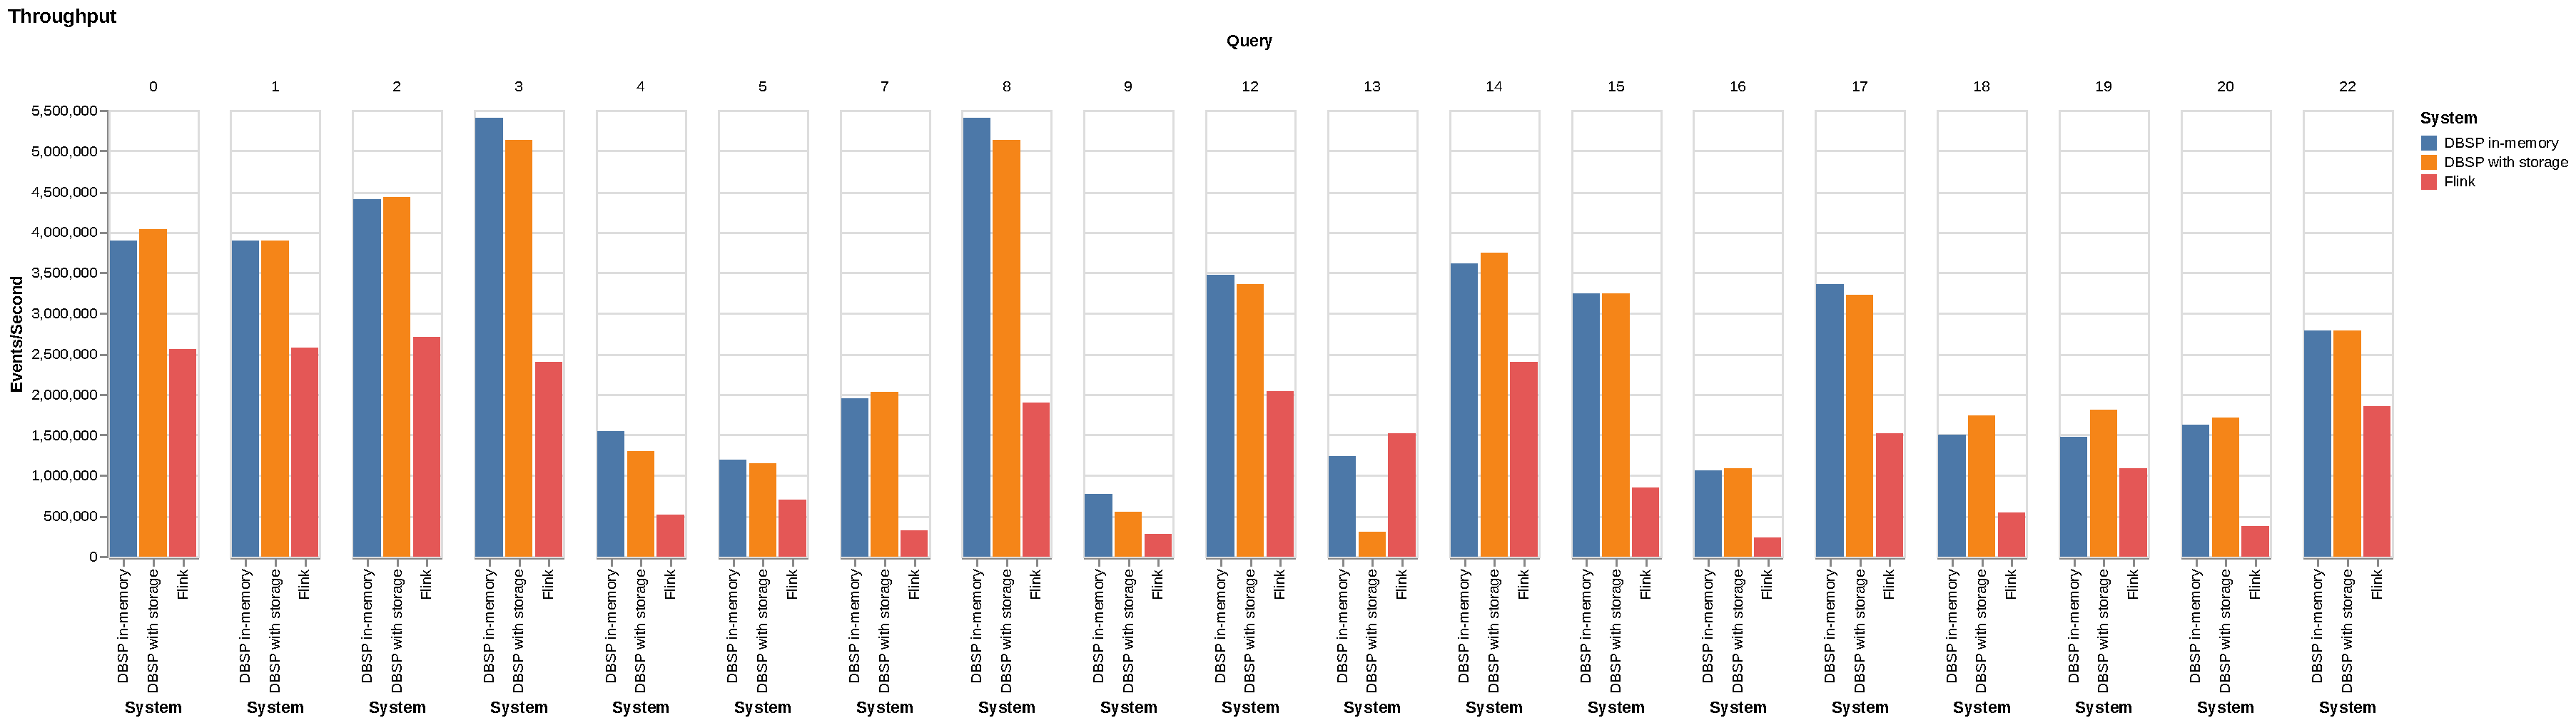
\includegraphics[width=.95\textwidth]{graph/throughput} \\
  (b) 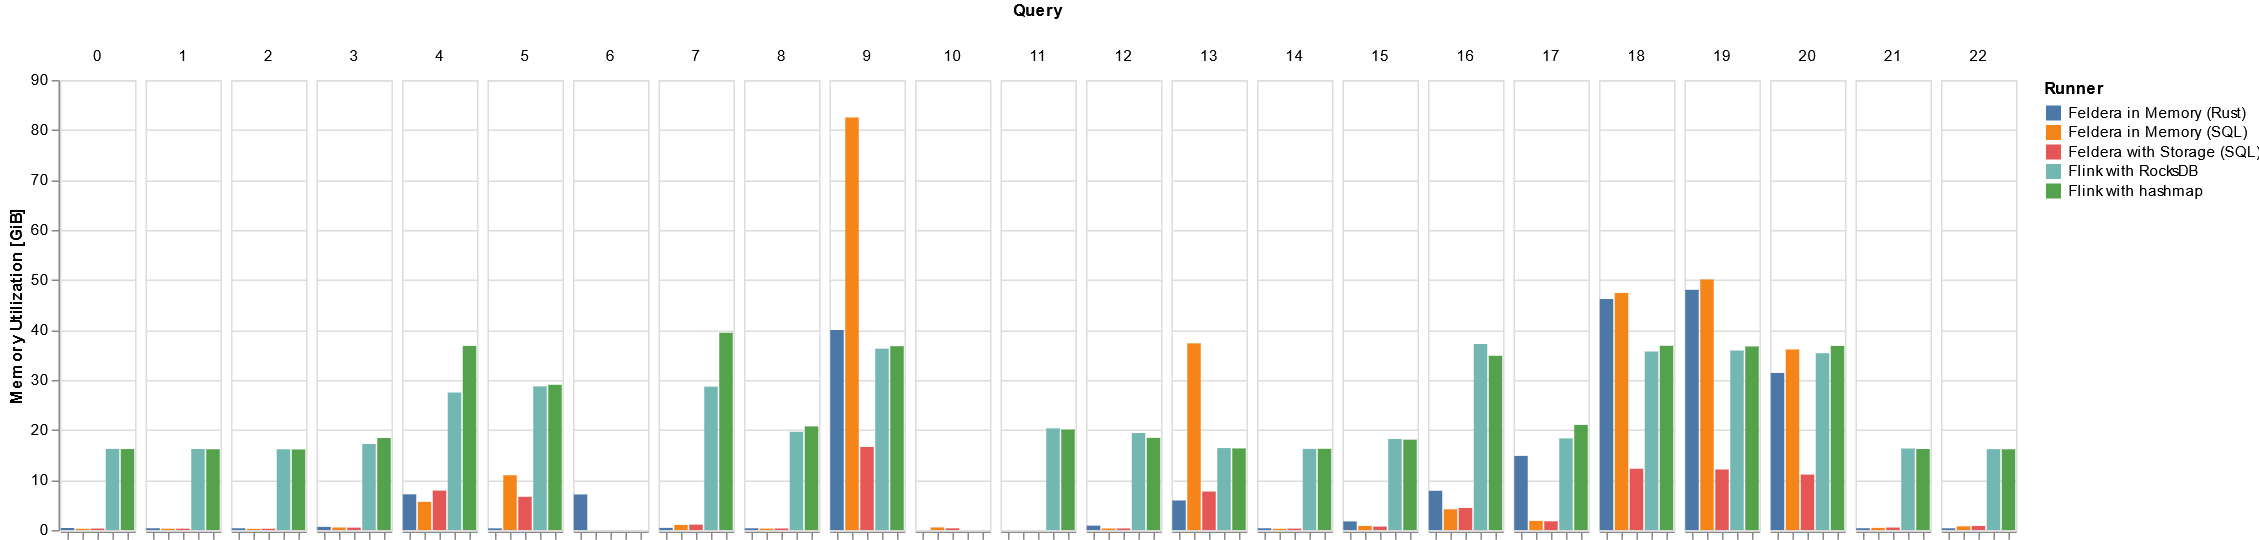
\includegraphics[width=.95\textwidth]{graph/memory} \\
  \caption{(a) Average throughput, in events processed per second, and
    (b) peak memory consumption, in GiB (\(2^{30}\) bytes), for the
    Nexmark queries that DBSP and Flink support in common, over
    100,000,000 events.\label{fig:macrobenchmark}}
\end{figure*}

\newcommand{\query}[1]{\textsf{#1}}

We compared DBSP against Flink on the Nexmark benchmark, which
consists of queries numbered \query{q0} through \query{q22}.  We
benchmarked the queries that the Flink and DBSP implementations
have in common.  We omitted \query{q6} because there was no Flink
implementation, and \query{q10} because we could not make Flink's
implementation for it work.  We omitted \query{q11} and \query{q21}
because DBSP does not yet support session windows and user-defined
functions.

We ran both the Flink and DBSP implementations on the same machine,
which has a 64-core, 128-thread Threadripper~3990X CPU and 256~GB RAM,
with Fedora Core~40 as the operating system. We present results for
100~million Nexmark events (input records), which is a moderate
number.

We ran DBSP as a single process configured with 16~worker threads and
otherwise with default settings.  We ran DBSP both with storage
disabled, where DBSP keeps all state in RAM, and with storage enabled,
where DBSP flushes state to secondary storage as it gets large
(see~\ref{sec:state-management}).  Enabling storage allows DBSP to
work with more state with less memory use, at some cost in throughput.

We configured the Flink implementation of Nexmark with the settings
recommended by the upstream project, running 8~Flink task manager
containers, each allocated 2~cores, and one Flink job manager
container.  We tried adjusting Flink and Nexmark settings, but none of
these changes improved Flink performance in a significant and
reproducible way.

DBSP and Flink support reading input from multiple kinds of data
sources.  For these measurements, we configured both of them to use
their own integrated Nexmark event generators, rather than pulling
them from Kafka or HTTP or another source.  This eliminated network
service performance and configuration as a possible source of
variability.

Figure~\ref{fig:macrobenchmark} reports our measurements.  The two
bars for DBSP in each case report results with and without enabling
secondary storage.


\paragraph{Throughput.}

\newcommand{\x}{\(\times\)}

Figure~\ref{fig:macrobenchmark}(a) shows throughput of DBSP versus
Flink.  In-memory Feldera is up to 6.2\x{} faster than Flink,
with a geometric mean of 2.2\x{} faster on average.  As queries
get more complicated, Feldera's advantage over Flink grows by a much
larger factor.  For example, \query{q7} is 6.2\x{} faster in
Feldera vs. Flink, and q16 and q20 are about 4.5\x{} faster.

\query{q13} is an outlier that performs slightly slower in Feldera
than Flink; with storage enabled, it is slower than Flink.  With
\query{q13} excluded, every remaining query runs at least
1.4\x{} faster in Feldera (with or without storage).  We are
investigating Feldera's performance with \query{q13}.

Storage generally has a small impact on throughput in Feldera, except
for \query{q13}, where it has about a 4\x{} penalty.

\query{q0} and other very simple queries perform about 1.5\x{} faster
with Feldera than Flink.

\paragraph{Peak memory.}

Figure~\ref{fig:macrobenchmark}(b) shows peak memory consumption of
DBSP versus Flink, as reported as the operating system RSS (resident
set size), for the Flink or Feldera processes.  For Feldera, this is a
single process; for Flink, it is the sum of the RSS in the 8 task
manager containers.  We did not include the control plane in either
case (in Feldera, the pipeline manager; in Flink, the job manager).

Feldera uses between 0.03\x{} and 2.6\x{} as much memory of Flink,
with a geometric mean of 0.24\x{}.

\query{q0} and several other queries use 2~GiB or less memory with Feldera,
but over 17~GiB with Flink.  These queries do not require Feldera to
store any state, or only minimal state, so it does not allocate much
memory.  Flink runs under the Java Virtual Machine, which might cause
it to allocate a high minimum amount of memory.

Most queries use less memory in Feldera than in Flink.  \query{q9} and
\query{q13} use substantially more, and \query{q18} and \query{q19}
use somewhat more, and in each case storage helps.
